The case study was done at Researcher's Night 2015 with two main objectives (i) cross-validate the findings obtained from the experiment, and (ii) use the Emotional Enrichment System to verify whether the participants would prefer scenes when the robot expresses emotions or rather moves without any emotion expression.

\subsection{Design and Setup}

This case study uses the results obtained in the experiment and was designed to have two parts (i) emotion expression through changes in linear velocity, angular velocity, oscillation angle, orientation and direction.  
(ii) Presentation of a small scene to verify whether the participants would prefer scenes when the robot shows emotions or not. the Emotional Enrichment System was used in both cases (with and without emotions). Two web-cams and eight Alvar tags were added to use Kalman filter to improve robots localization in the stage. The detection of the AR tags is done through the use of the ROS package ar\_track\_alvar~\cite{artag2015}. The distribution of the web-cams and the tags are depicted in Figure~\ref{fig:setup_fourth}. 

\begin{figure}
	\centering
	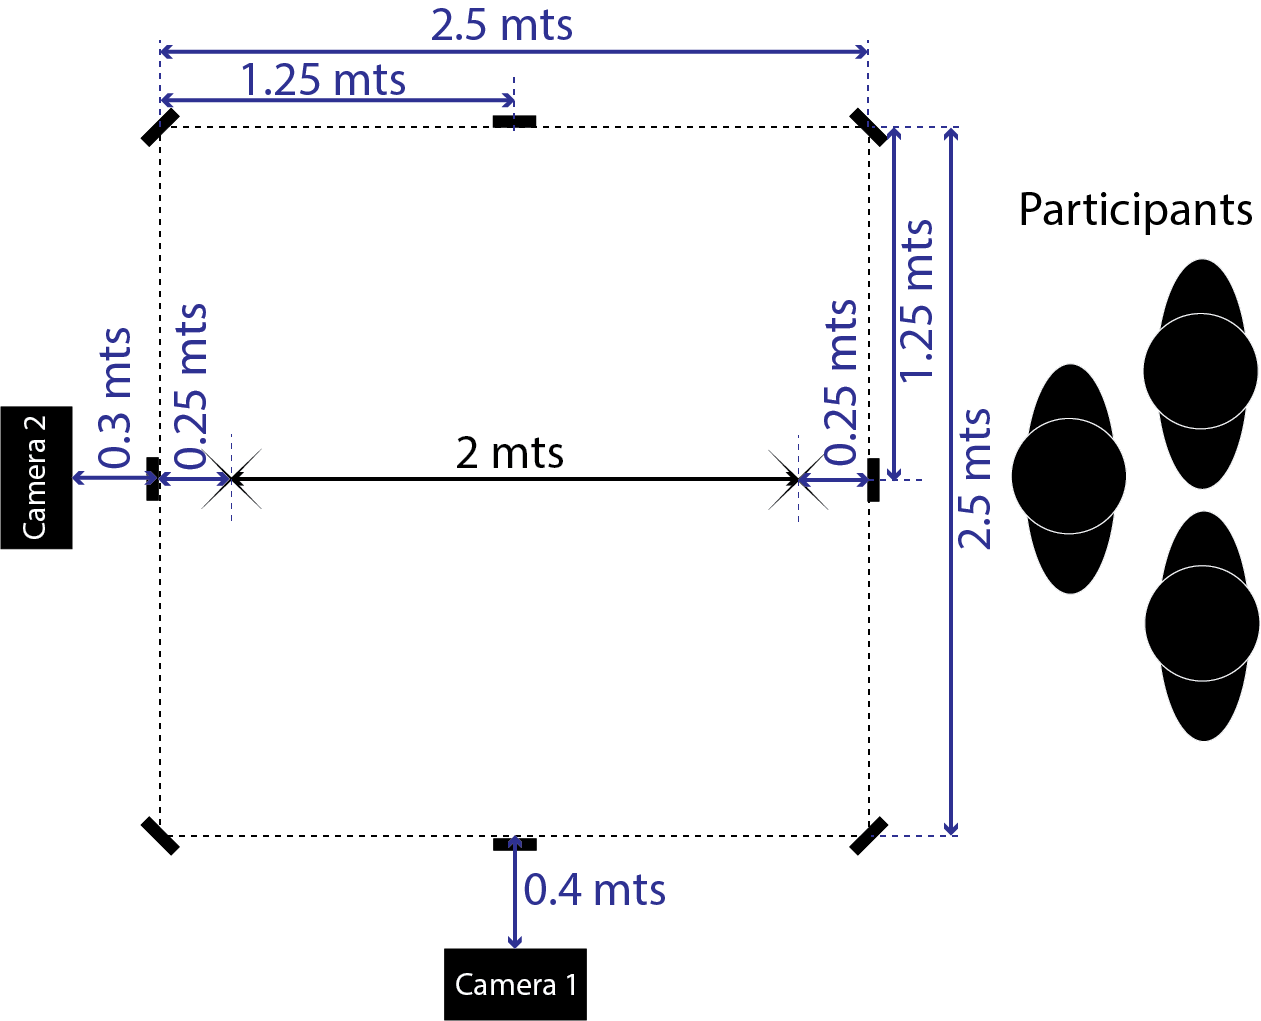
\includegraphics[width=0.45\textwidth]{./Images/FourthCase.png} 
	\caption{Environment setup for the case study.}
	\label{fig:setup_fourth}
\end{figure}

\subsubsection{Emotion Description}

The parameters selected for each of the four emotions (\textit{Anger}, \textit{Happiness}, \textit{Sadness} and \textit{Fear}) are shown in Table~\ref{table:selected_fourth}. The main considerations to select the two implementations for each emotion were: (i) the linear velocity should be greater than $0$. In other words the robot should show some linear displacement. And (ii) it should be in the top 10 list of the emotion obtained in the experiment.

\begin{table}[h]
\centering
\small
\caption{Parameters' values selected from the experiment.}
		\label{table:selected_fourth}
		\begin{tabular}{|c|p{0.9 cm}|p{0.9 cm}|p{0.9 cm}|p{1.05 cm}|p{0.9 cm}|}
			\hline
%\rotatebox{90}{\textbf{Emotion } }&
%\rotatebox{90}{\textbf{Direction  ($rad$)}}&
%\rotatebox{90}{\textbf{Orientation ($rad$)} }&
%\rotatebox{90}{\textbf{Linear Velocity ($mm/s$) }}&
%\rotatebox{90}{\textbf{Angular Velocity ($rad/s$) }}&
%\rotatebox{90}{\textbf{Angle ($rad$)}}\\	
\textbf{Emotion}&\textbf{Direc-tion  ($rad$)} & \textbf{Orien-tation ($rad$)} & \textbf{Linear Velocity ($mm/s$) } & \textbf{Angular Velocity ($rad/s$) } & \textbf{Angle ($rad$)} \\
			\hline
			Happiness 1&$0$&$0$&$500$&$3$&$0.349$\\
			\hline
			Happiness 2&$0$&$0$&$900$&$3$&$0.174$\\
			\hline
			Anger 1&$\pi$&$0$&$500$&$3$&$0.087$\\
			\hline
			Anger 2&$0$&$0$&$900$&$1$&$0.087$\\
			\hline
			Fear 1&$\pi$&$\pi$&$900$&$2$&$0.174$\\
			\hline
			Fear 2&$\pi$&$\pi$&$500$&$2$&$0.087$\\
			\hline
			Sadness 1&$\pi$&$0$&$200$&$1$&$0.349$\\
			\hline
			Sadness 1&$0$&$\pi$&$200$&$1$&$0.349$\\
			\hline
			\end{tabular}
\end{table}


\subsubsection{Scene}
%TODO change this part of the text and give some information about this, and  motivate its use, which bassically is to verify the emotional enrichment system
As it was already mentioned, actors should adapt to different circumstances during the performance. Following this approach, the stage was discretized in 9x9 matrix as is shown in Figure~\ref{fig:stage_division}. Thus, the movements of the robot are given in terms of the matrix positions. This allows the adaptation to different stage dimensions because the robot's final position is calculated by the Emotional Enrichment System during execution taken under consideration the stage dimensions. For instance, during the scene's preparation in the laboratory the stage was 3 meters per 3 meters, but in the final presentation the stage was 2.5 meters per 2.5 meters.

\begin{figure}
	\centering
	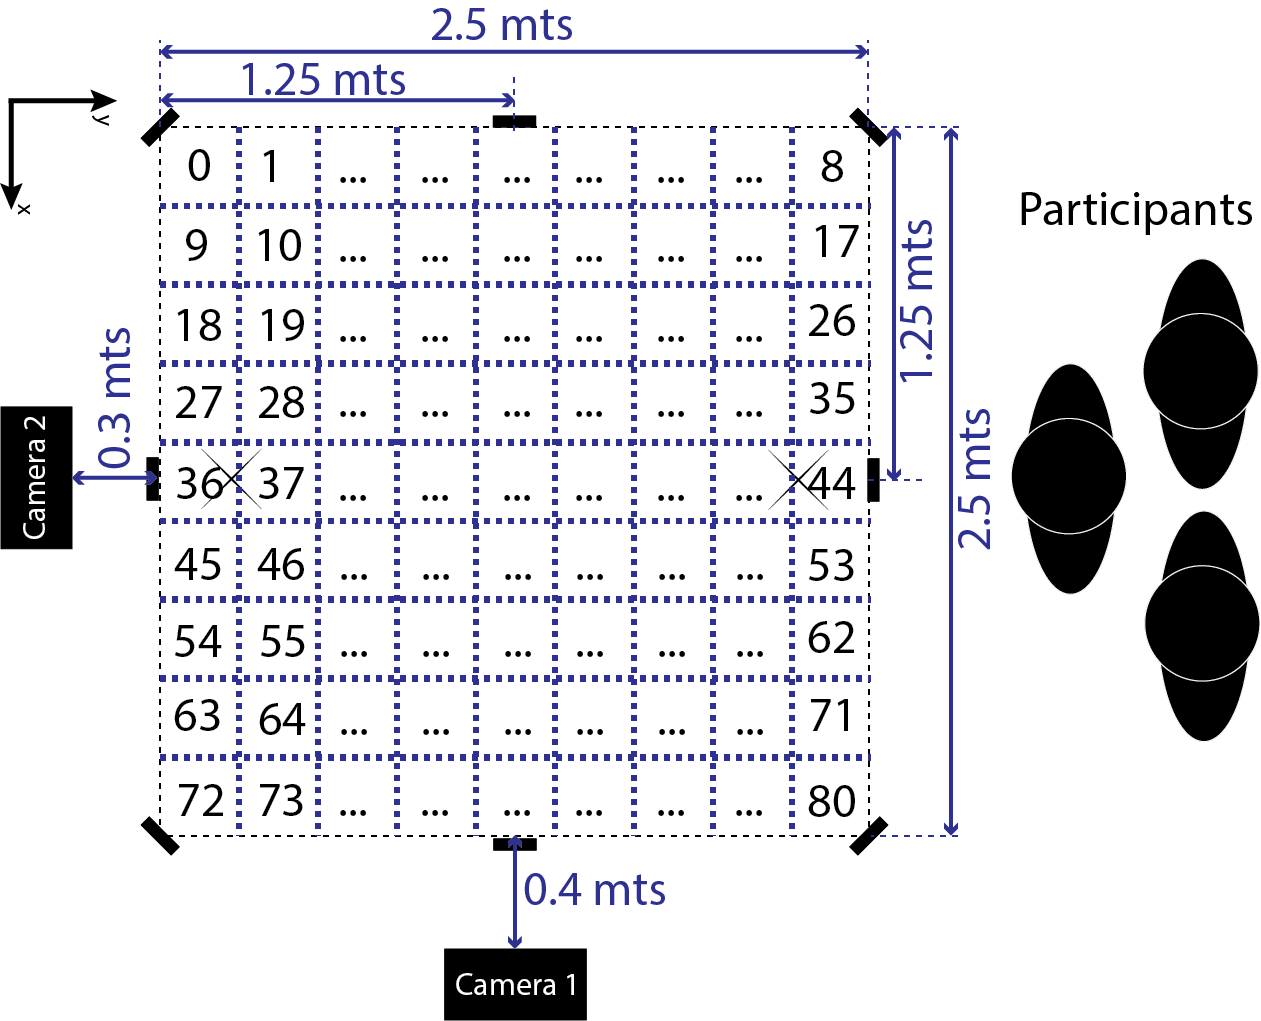
\includegraphics[width=0.45\textwidth]{./Images/FourthCaseScene.png} 
	\caption{Stage discretization  used for the small scene. The blue squares correspond to the each zone, while the numbers correspond to the ID given to each zone.}
	\label{fig:stage_division}
\end{figure} 
%TODO Change this paragraph and motivate the reason this is important and instead of puting the figures, write the references to those figures
The scene's description is the following: the robot starts in the middle of the stage to move to the upstage right (Figure~\ref{fig:StageDirections}), close to the right wing. Then, the robot moves to upstage right center and rotates by $\pi/2$ left (Figure~\ref{fig:BodyPosition}). Next the robot moves to the right center to then go to the center. When it arrives there, it turns full back and move backwards to downstage center with a full front orientation. There, it turns full back to move to center. Finally the robot turns to profile right and it does a step back; then it goes to the upstage center and then upstage right. The sequence of movements programmed to the robot are depicted in Figure~\ref{fig:movement}.
\begin{figure*}
	\centering
	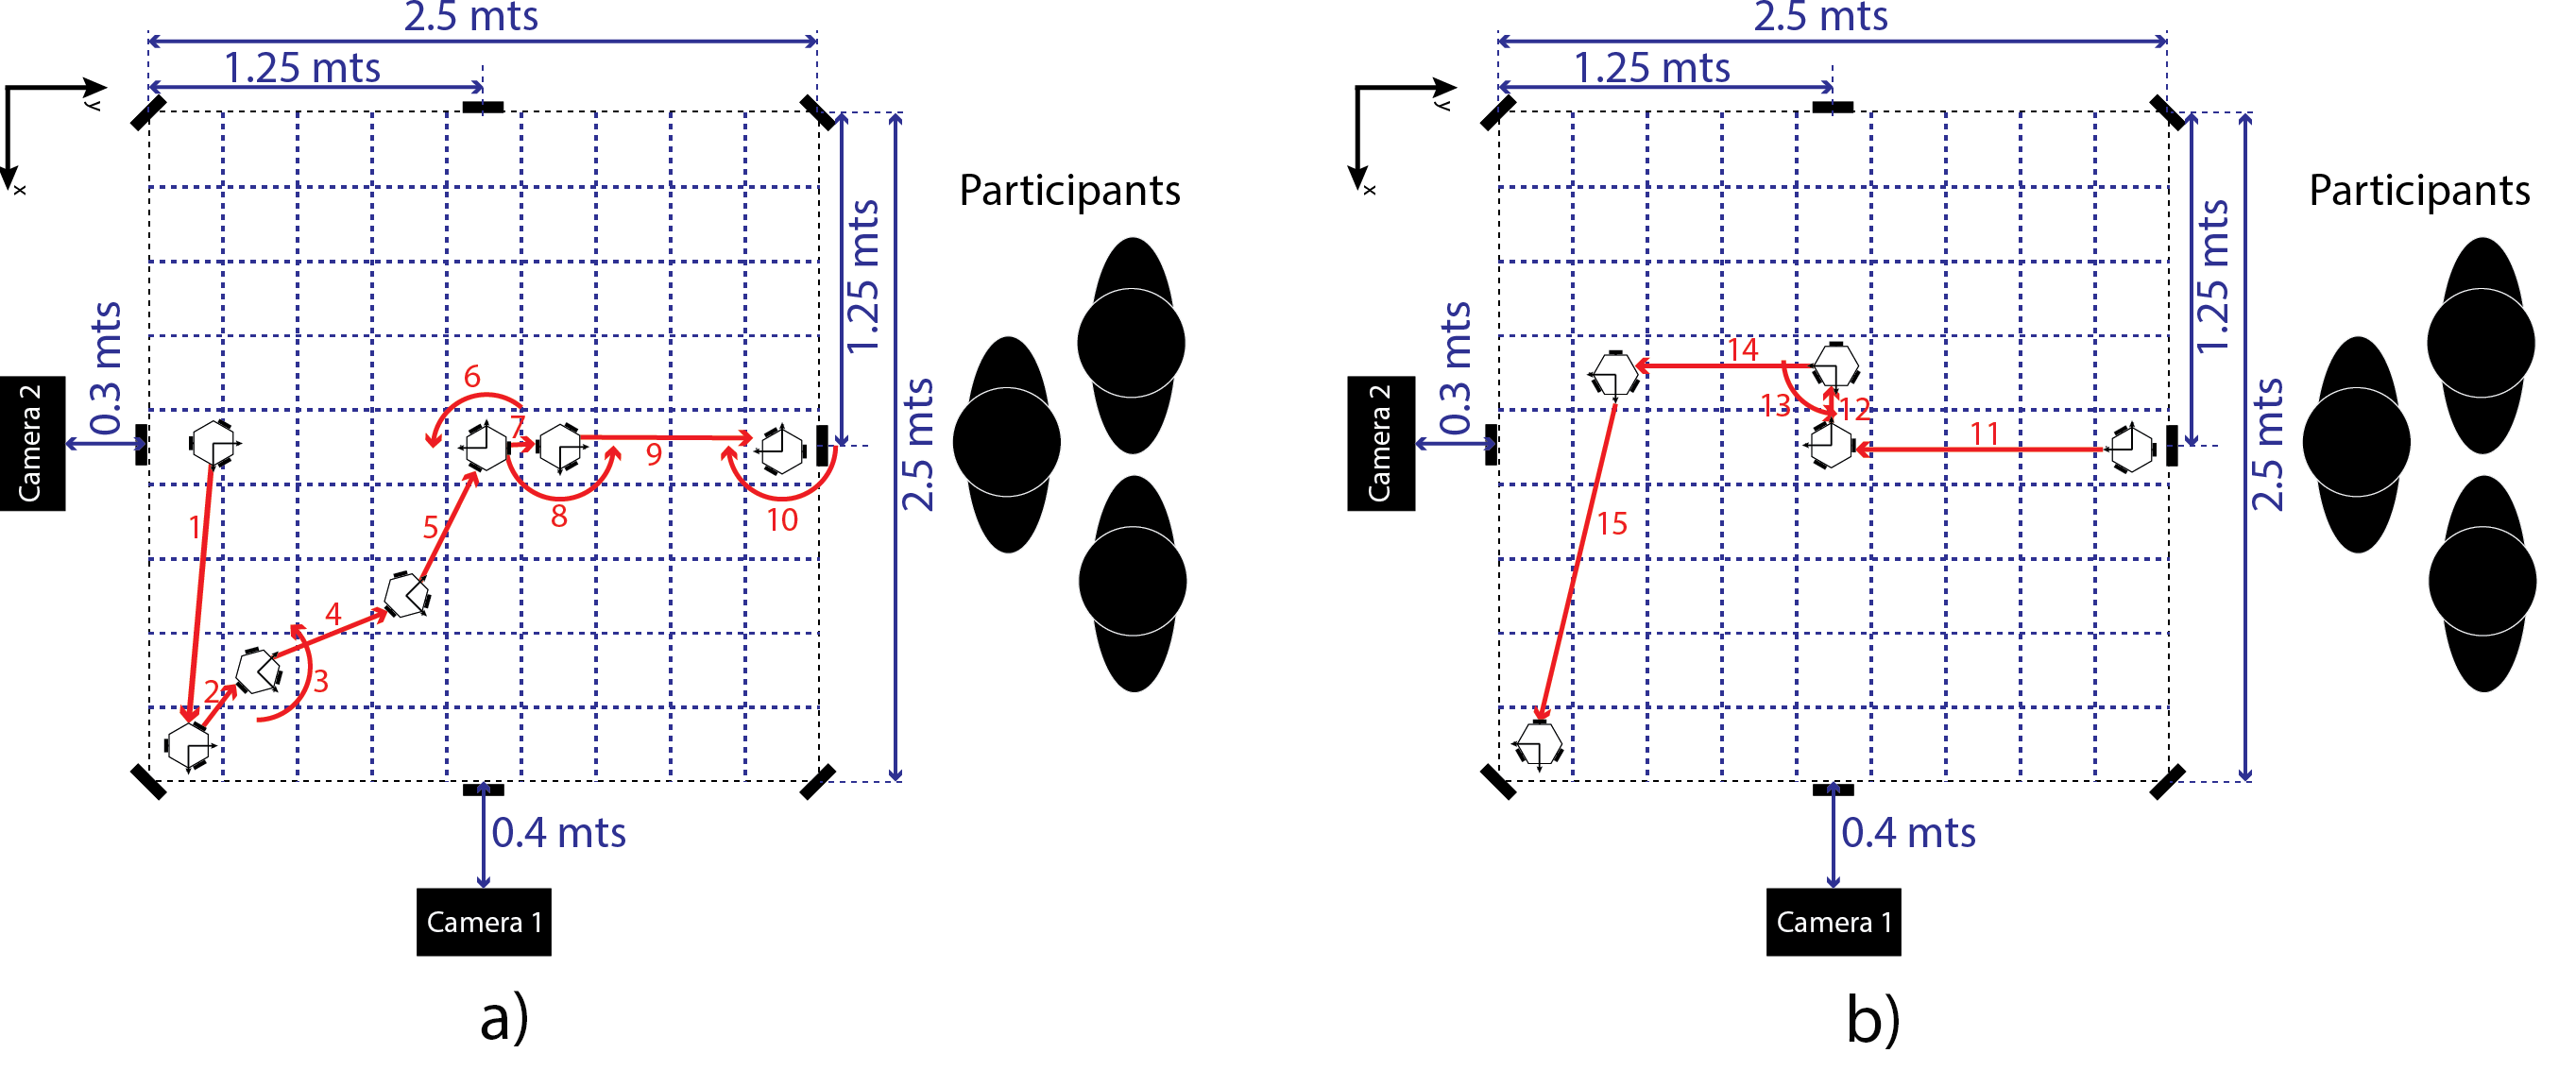
\includegraphics[width=0.85\textwidth]{./Images/fourthCaseSceneD.png} 
	\caption{Sequence of movements done by the robot. The red arrows show the trajectory done by the robot, while the numbers show the order among the movements. a) The first ten movements b) The last five movements }
	\label{fig:movement}
\end{figure*}

The relation between emotion and movement is as follow: movements one, two, three, four and five are expressed without any emotion. Movements six, seven, eight, nine and ten show fear. Movement eleven depicts happiness, and the remaining movements depict sadness. The two scenes are executed by the Emotional Enrichment System using the same ''script'' and the emotion selection is done manually via graphical interface (Figure~\ref{fig:graphical_interface}).The ''script'' were written in JSON using the language described in the Section~\ref{}.

\begin{figure}
	\centering
	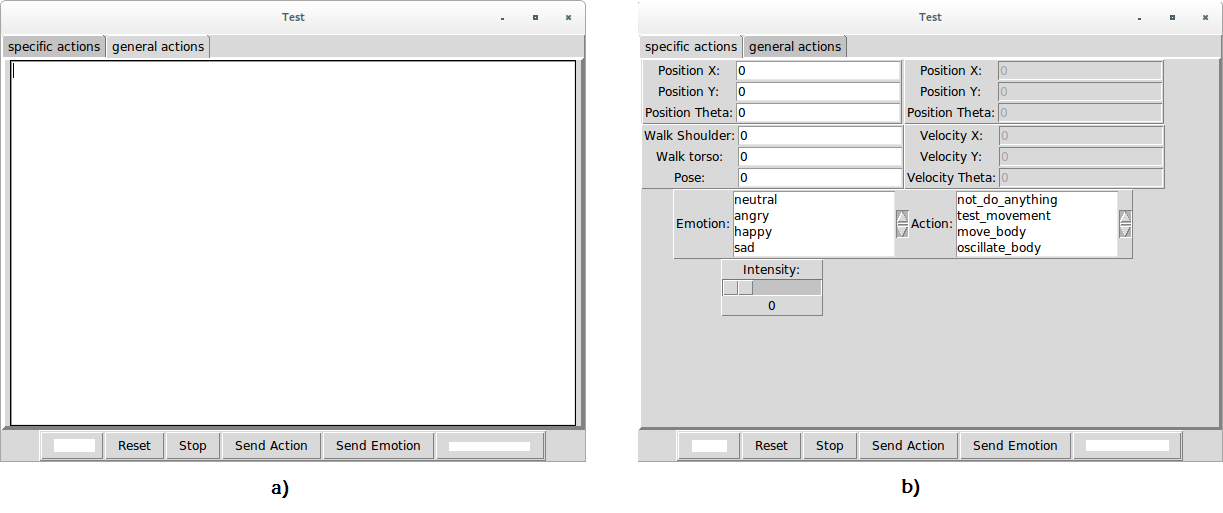
\includegraphics[width=0.45\textwidth]{./Images/InterfaceExperiment.png} 
	\caption{Graphical interface used to communicate with the Emotional Enrichment System. a) It is the interface used to send the actions sequence. b) It is the interface used to send a emotion and its intensity.}
	\label{fig:graphical_interface}
\end{figure}

\subsection{Study}

This case study was done during Researchers' Night, 2015. During a period of two days, people were asked to participate to this study. Each subject was exposed to two rounds, in each one the robot was performing a different emotion. And  they were also exposed twice to a small scene, one with emotion and other without emotions. The emotions showed in each trial and the order of the scenes (with or without emotion) were generated randomly beforehand. The total number of volunteers was 256: 128 males, 126 females, and 2 that chose not to specify their gender. The average age was 27.29 years, with standard deviation of 16.58, minimum age was 4 and maximum 76.
